\pagebreak
\section{Auf- und Ab sitzen}
	Fahrzeuge werden in umgekehrte Trupp Reihenfolge betreten. (Siehe auch \nameref{para:fahrzeug-betreten})
	
\subsection{Sicherungsbereich}
	Der Sicherungsbereich nach Verlassen des Fahrzeuges entspricht den Standsicherungsbereichen für  Trupps (siehe \nameref{subsec:360sicherung}, \autoref{subsec:360sicherung}). Mehrere Trupps können sich z.\,B. 180° Sicherungsbereiche abstimmen. \\
	Kommando Verlassen: Alle Truppteile verlassen das Fahrzeug \\
	Kommando Absitzen: Schütze bleibt, Fahrer bleibt im Fahrzeug bzw. in der Nähe des Fahrzeuges, restliche Personen verlassen das Fahrzeug und bauen Sicherung auf.\\
	
	Wichtig:
	\begin{itemize}
		\item Bewegungskorridor vor und hinter dem Fahrzeug immer frei lassen\\ 12 Uhr ist immer die Fahrzeugfront
		\item Ein Fahrzeug in ARMA ist keine Deckung, wenn der Gegner AT-Waffen besitzt
		\item Abstand halten:\\ Wenn nicht anders befohlen, 20 Meter Abstand vom Fahrzeug\\ Fahrzeuge tendieren zum Explodieren, bieten schlechte Deckung und brauchen zudem jederzeit Platz für Manöver
	\end{itemize}
	\begin{figure}[htbp]
		\centering
		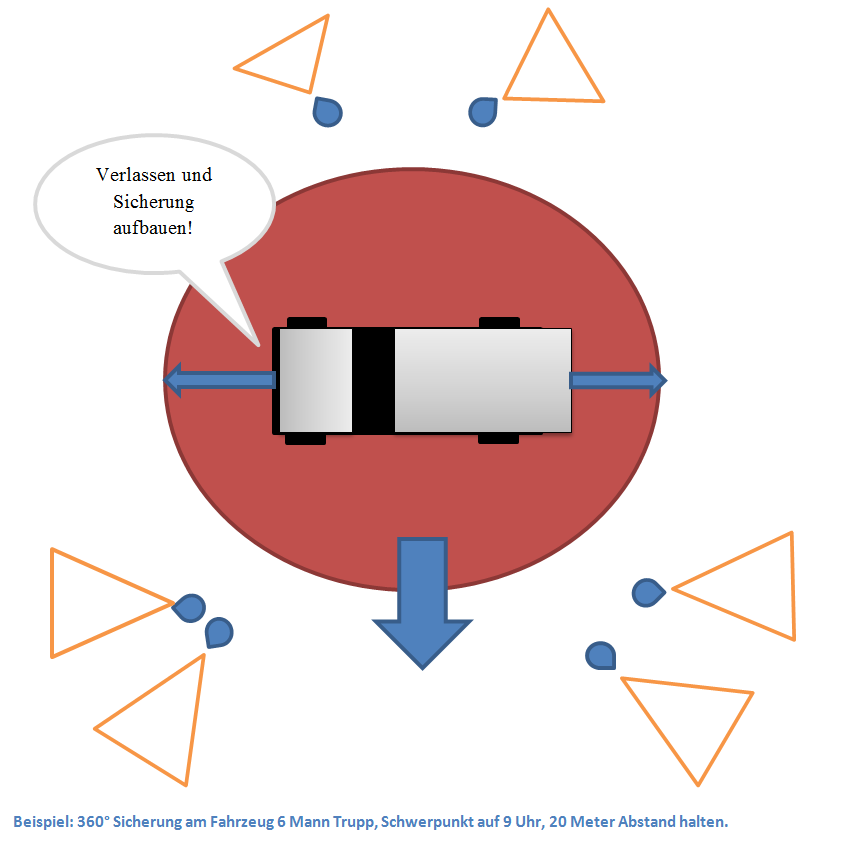
\includegraphics[width=15cm]{./img/grundlagen/umgangMitFahrzeugen/Fahrzeug_verlassen.png}
		\caption{Absitzen und Sicherung beim Fahrzeug}
	\end{figure}
